\begin{figure*}[hbtp]
  \centering
  \subfigure[Results of each graph]{
    \label{fig:hybrid--all}
    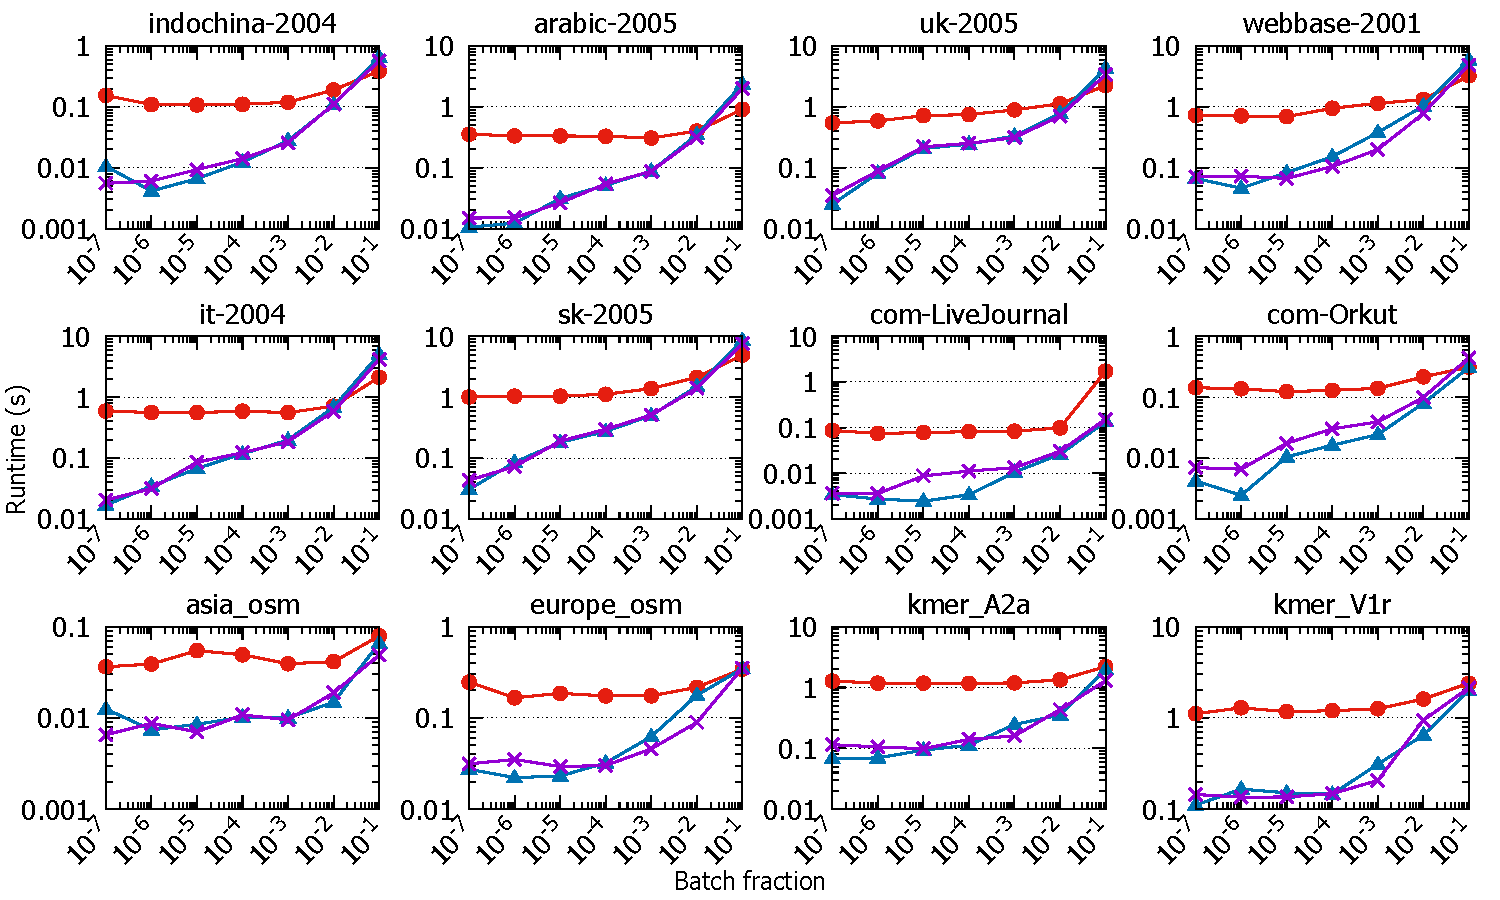
\includegraphics[width=0.58\linewidth]{out/hybrid-all-fullx.pdf}
  }
  \subfigure[Overall result]{
    \label{fig:hybrid--am}
    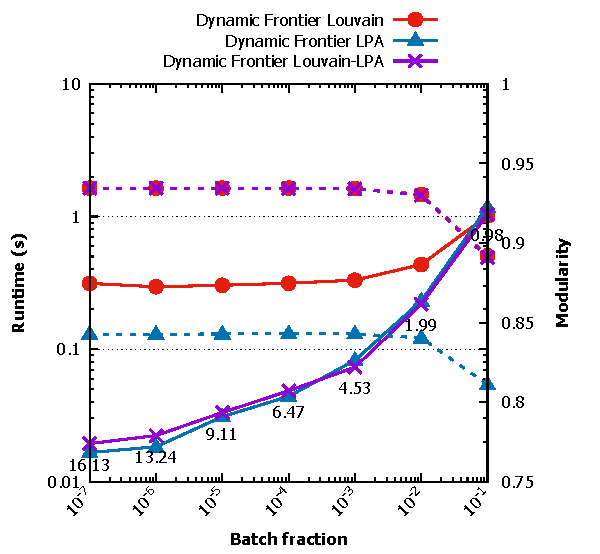
\includegraphics[width=0.38\linewidth]{out/hybrid-am.pdf}
  } \\[-2ex]
  \caption{Time taken (solid lines), and modularity of communities obtained (dashed lines) along the right Y-axis, with \FroLou{}, \FroLPA{}, and \FroHyb{} (Algorithms \ref{alg:louvain}, \ref{alg:rak}, and \ref{alg:hybrid}) on batch updates of increasing size from $10^{-7} |E|$ to $0.1 |E|$. Note that both axes are logarithmic. Speedup of \FroHyb{} with respect to \FroLou{} is labeled.}
  \label{fig:hybrid}
\end{figure*}
